\chapter{Інтервенційні втручання}


\section{Які є види інтервенційних втручаннь на печінці?}
Інтервенційні втручання - група мініінвазивних методик, що використовують в якості допоміжного або самостійного метода локорегіонального лікування патології печінки.  Як правило такі втручання виконують під ангіографічним, рентген, УЗД або КТ контролем.

До них відносять:
\begin{itemize}
    \item Ендоваскулярні методики
    \begin{itemize}
        \item трансартеріальна хемоемболізація пухлин - локальна хіміотерапія, коли медиамент доставляється безпосередньо до пухлини через печінкову артерію)
        
        \begin{marginfigure}%
            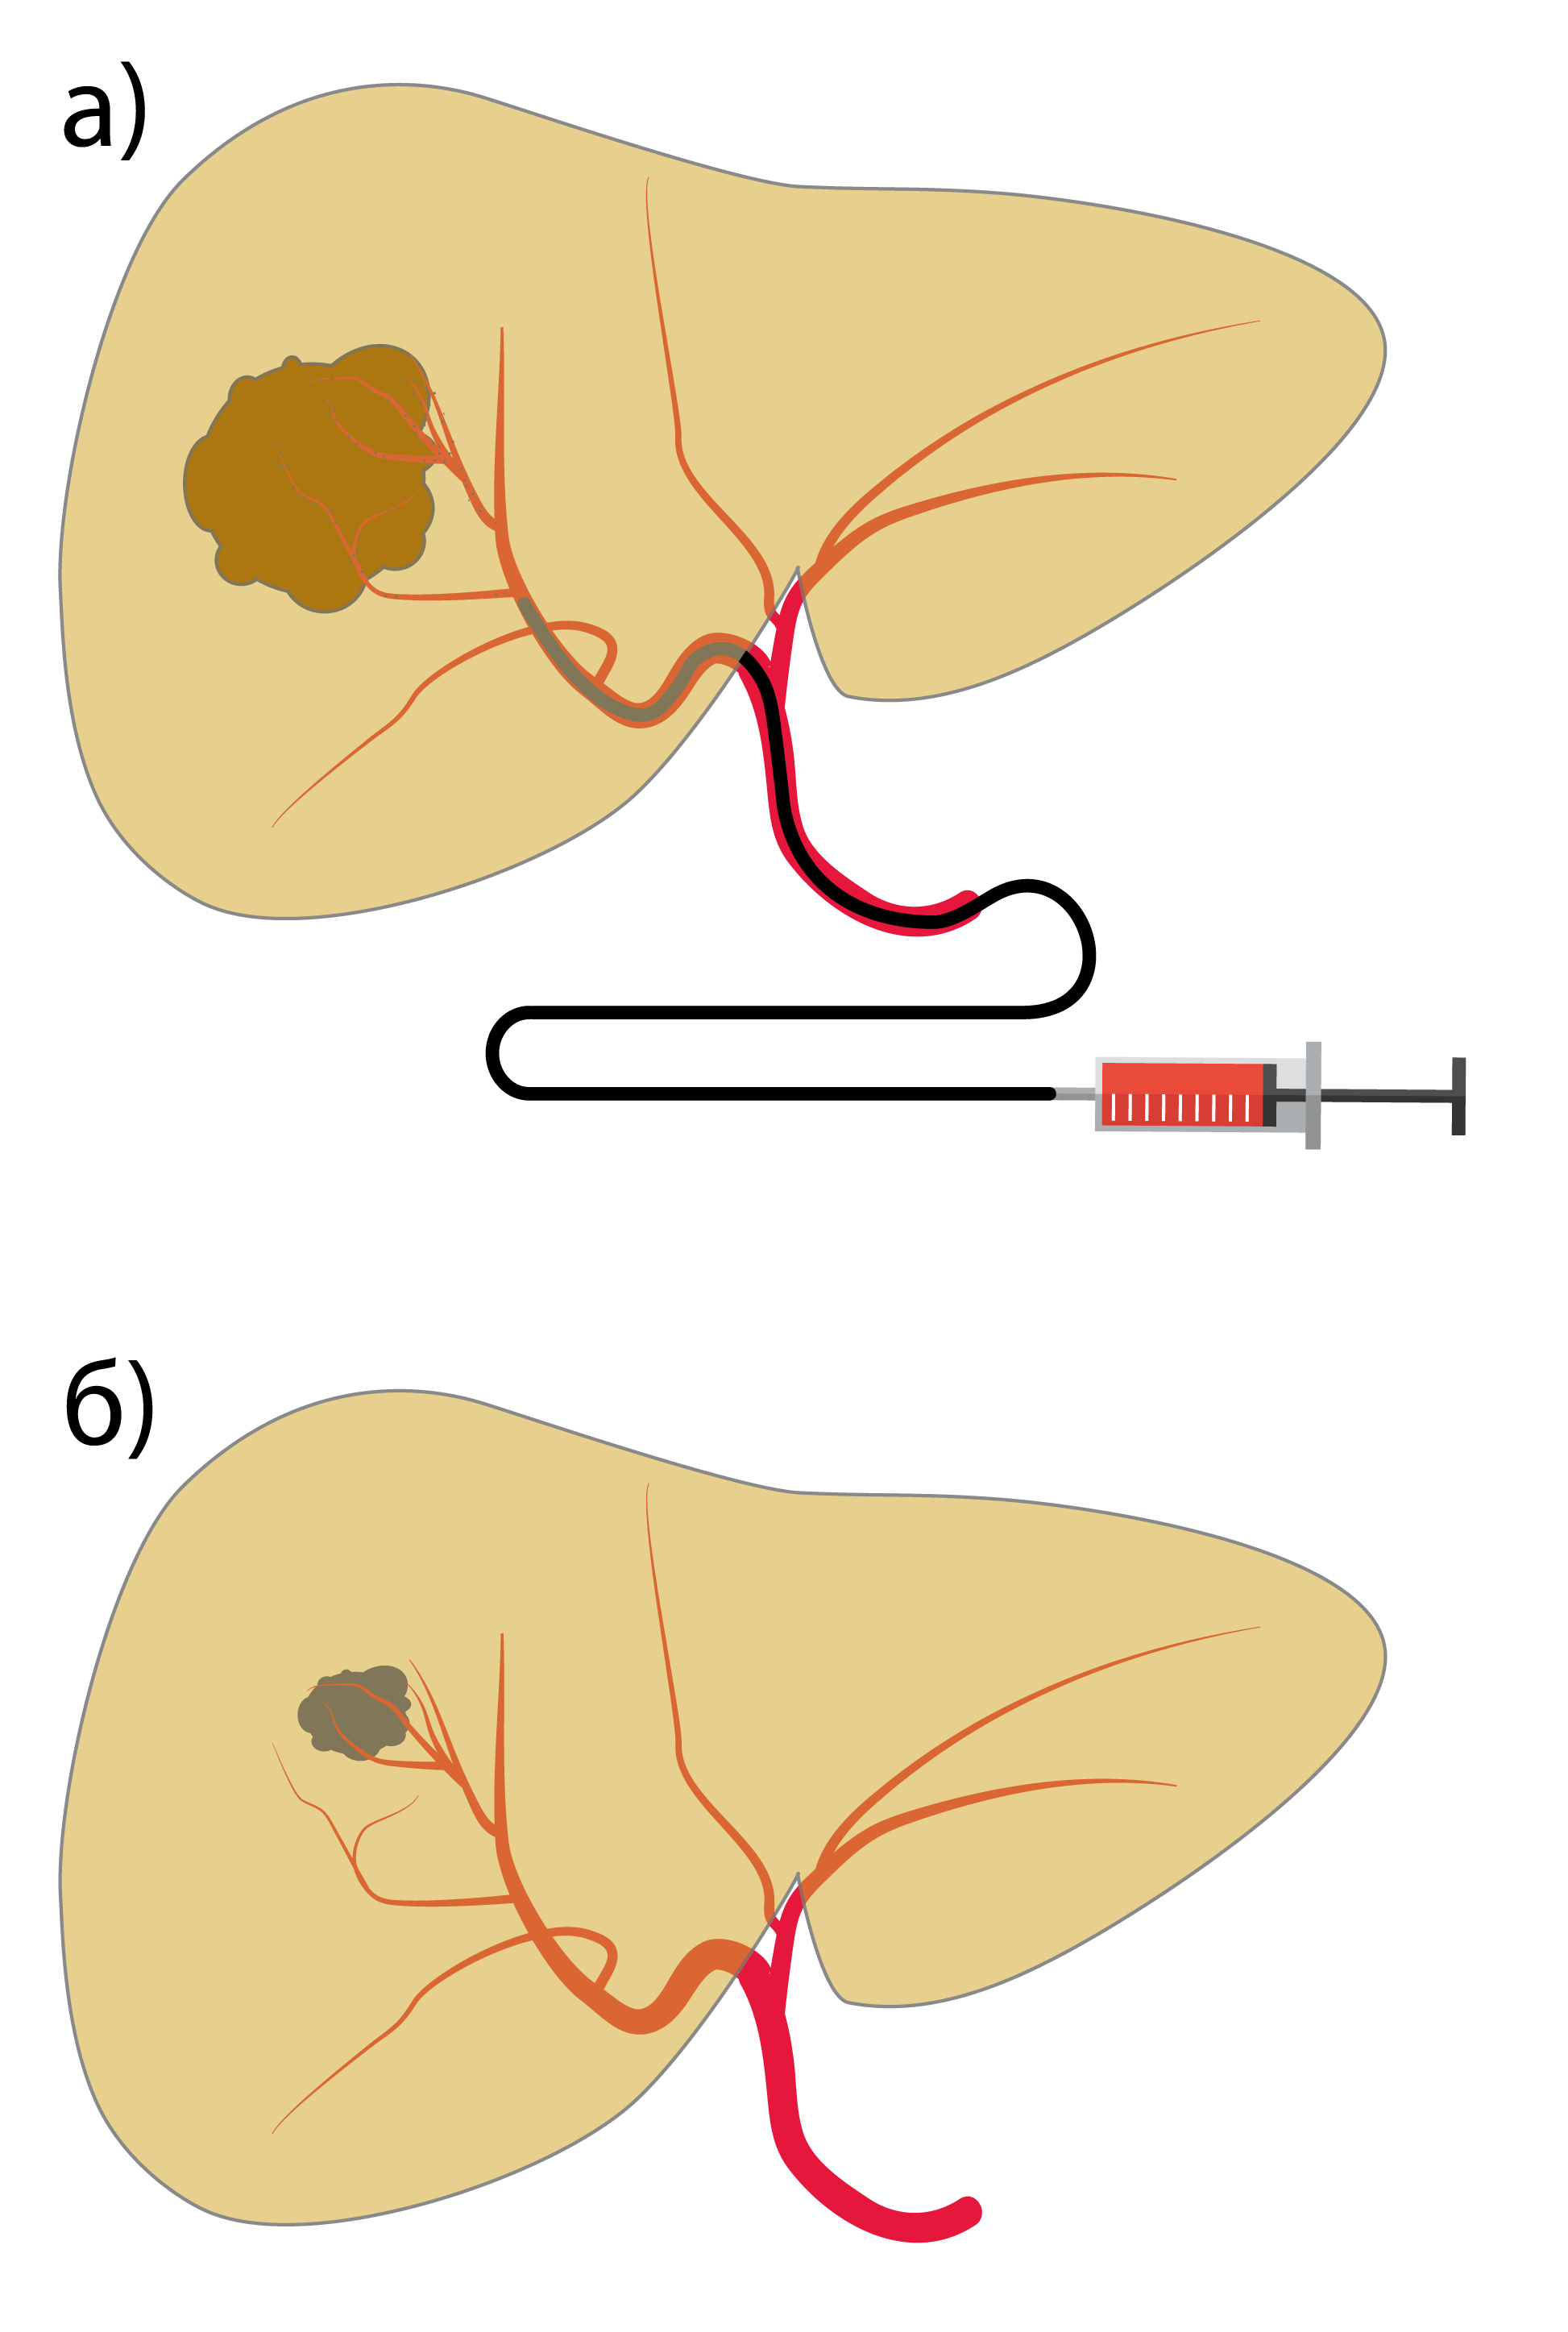
\includegraphics[width=\linewidth]{Figures/TACE_Vertical.png}
            \caption{Трансартеріальна хемоемболізація печінкової артерії (TACE) а) хіміопрепарат вводиться безпосередньо в пухлину через гілку печінкової артерії б) зменьшення та некроз пухлини через 1 місяць }
            \label{fig:goalbladder}
        \end{marginfigure}
        
        \item емболізація ворітної вени - ендоваскулярна процедура перекриття кровотоку по ворітній вені до пухлини. Застосовується в якості передопераційної підготовки для збільшення печінкового залишку перед виконанням резекції печінки
        
        \begin{marginfigure}%
            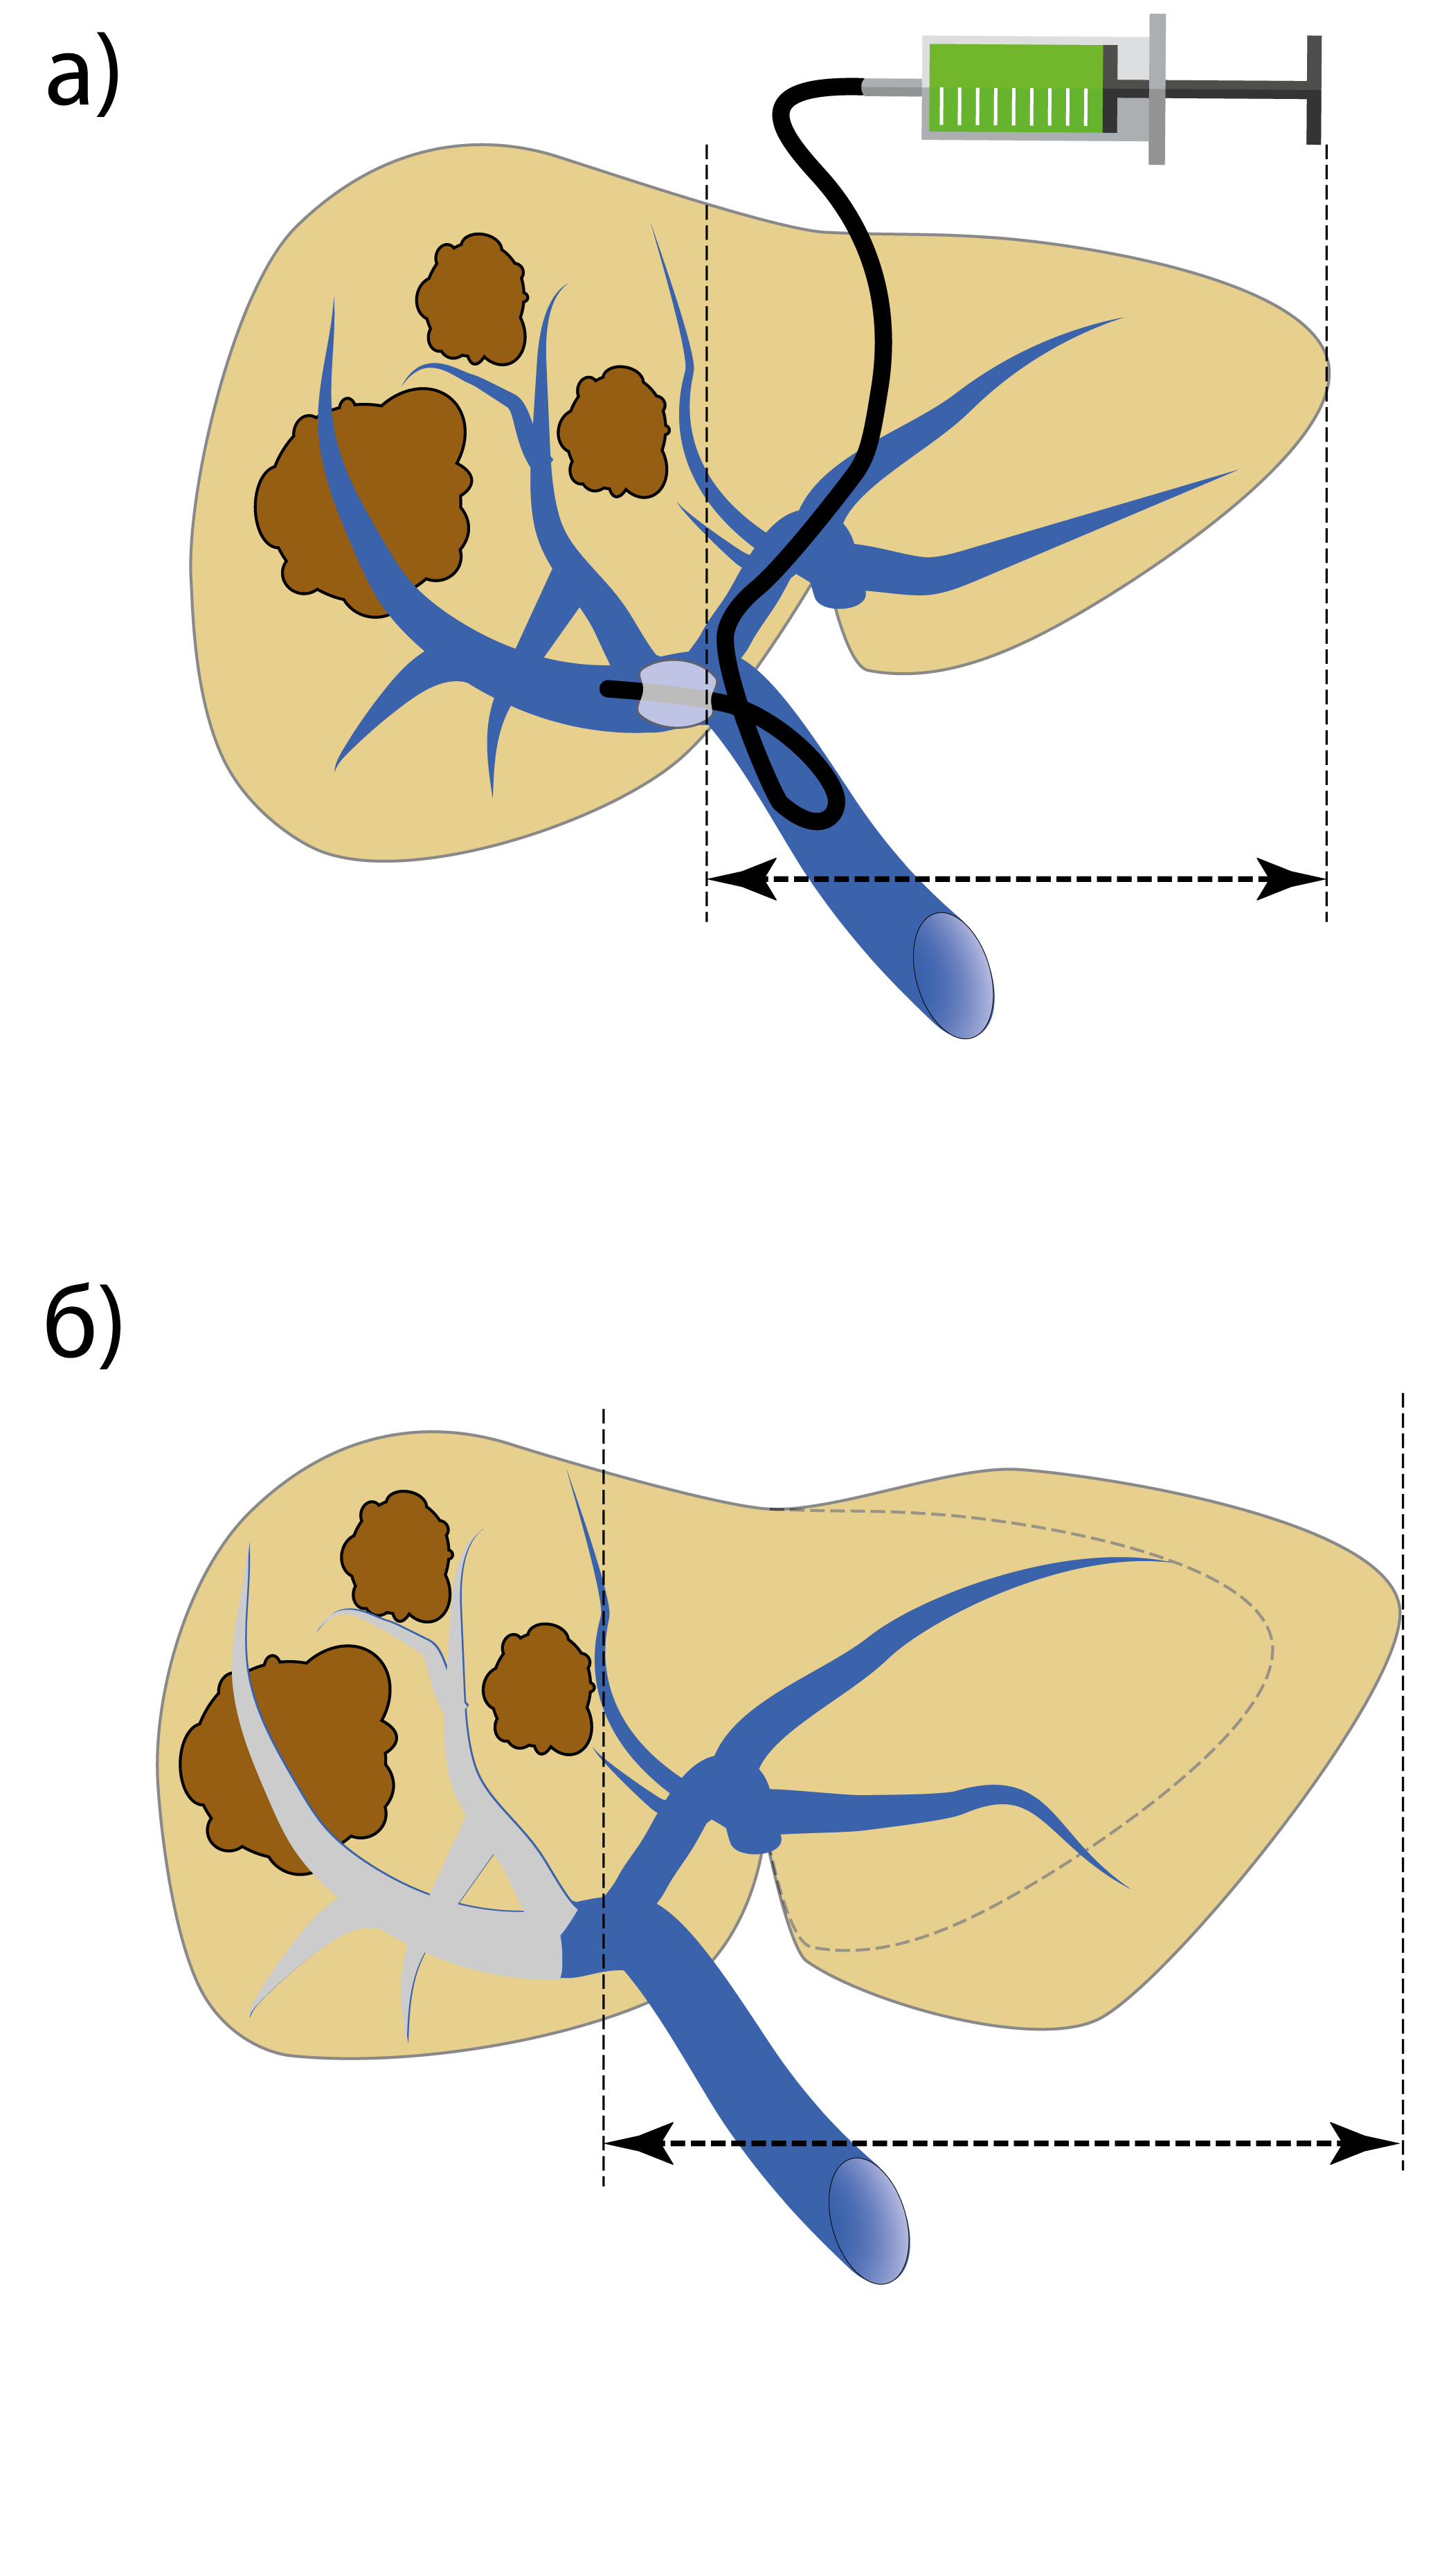
\includegraphics[width=\linewidth]{Figures/PVE_Vertical.png}
            \caption{Емболізація ворітної вени. а) мікроемболи вводяться в просвіт ворітної вени для перекриття кровотоку на уражену частину печінки б) збільшення потенційного печінкового залишку через 3-4 тижні }
            \label{fig:goalbladder}
        \end{marginfigure}
        
    \end{itemize}
    \item УЗ-контрольовані втручання
    \begin{itemize}
        \item абляція пухлин новоутвореннь печінки - знищення пухлини за допомогою локальної дії змінного електричного високочастотного струму, радіохвиль чи етанолу. Виконується під УЗ- або КТ- контролем 
        \begin{marginfigure}%
            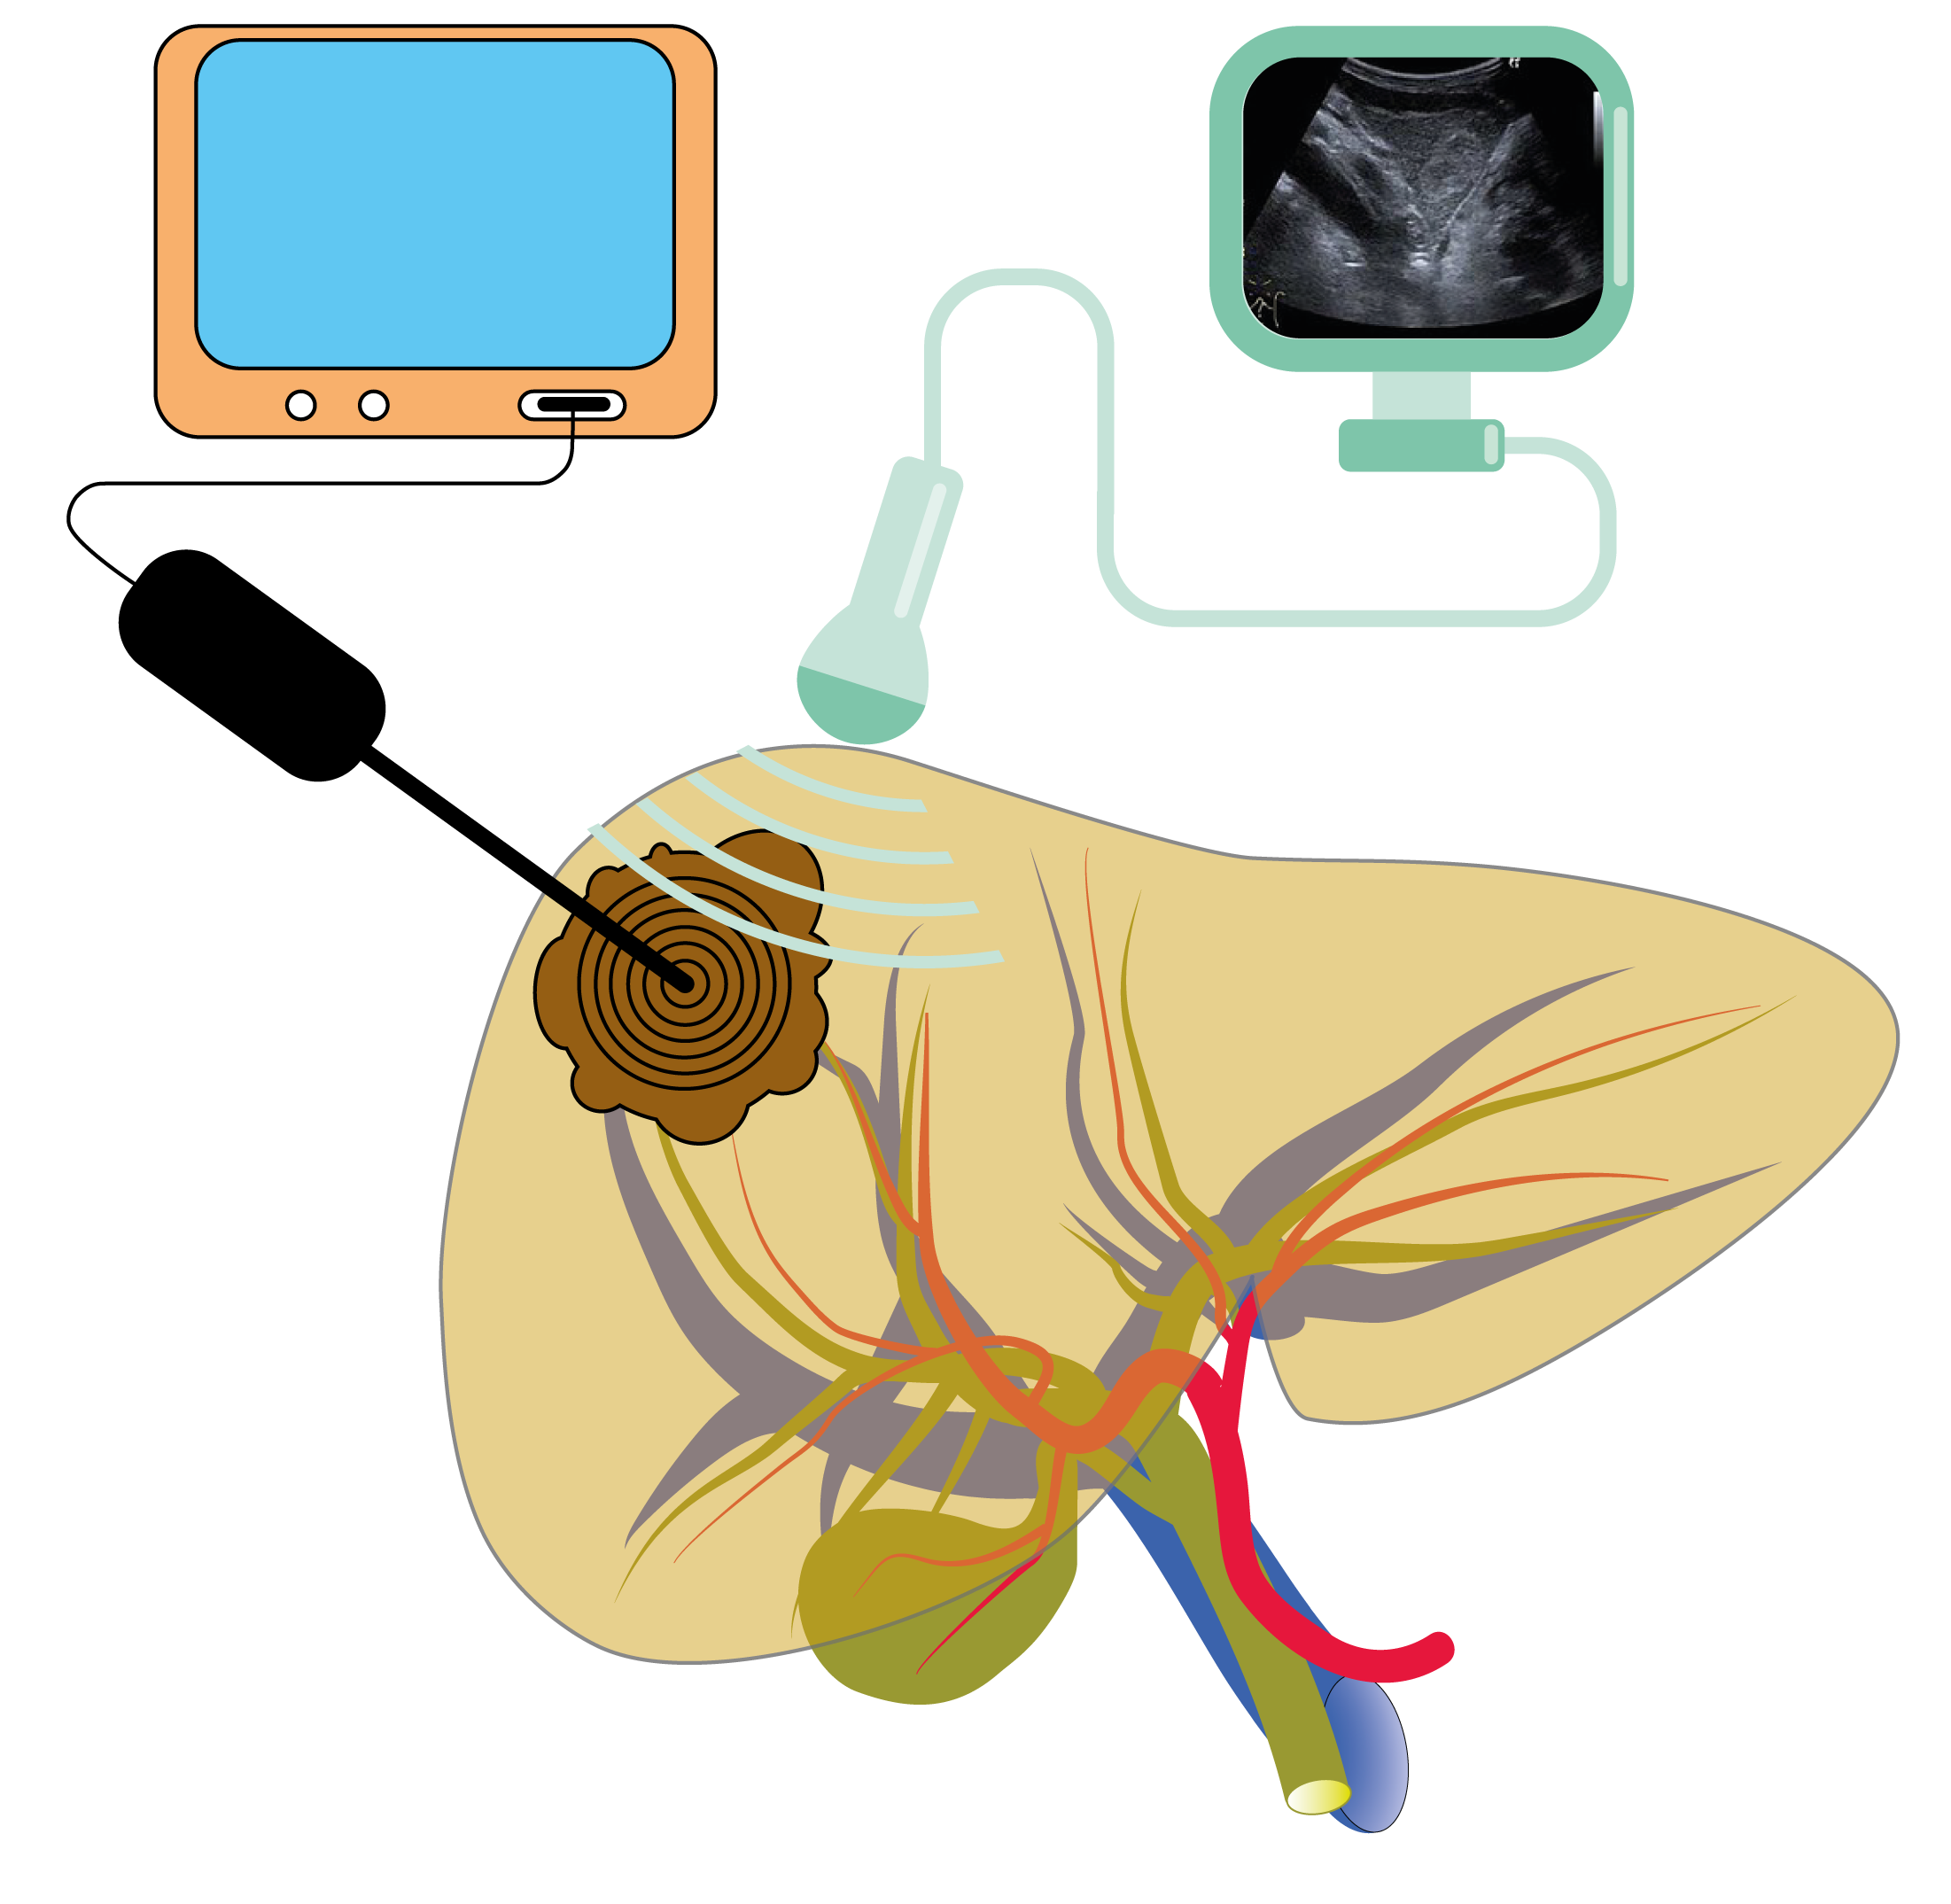
\includegraphics[width=\linewidth]{Figures/US procedures_Ablation.png}
            \caption{Високочастотна абляція пухлини. Під дією змінного тока високої частоти на кінці введеного під контролем ультразвуку електрода вогнище піддається термічній деструкції }
            \label{fig:goalbladder}
        \end{marginfigure}
        
        \item пункція та дренування кіст - евакуація вмісту кісти під УЗ-контролем та встановлення дренажної трубки в її порожнину за необхідності
        
        \begin{marginfigure}%
            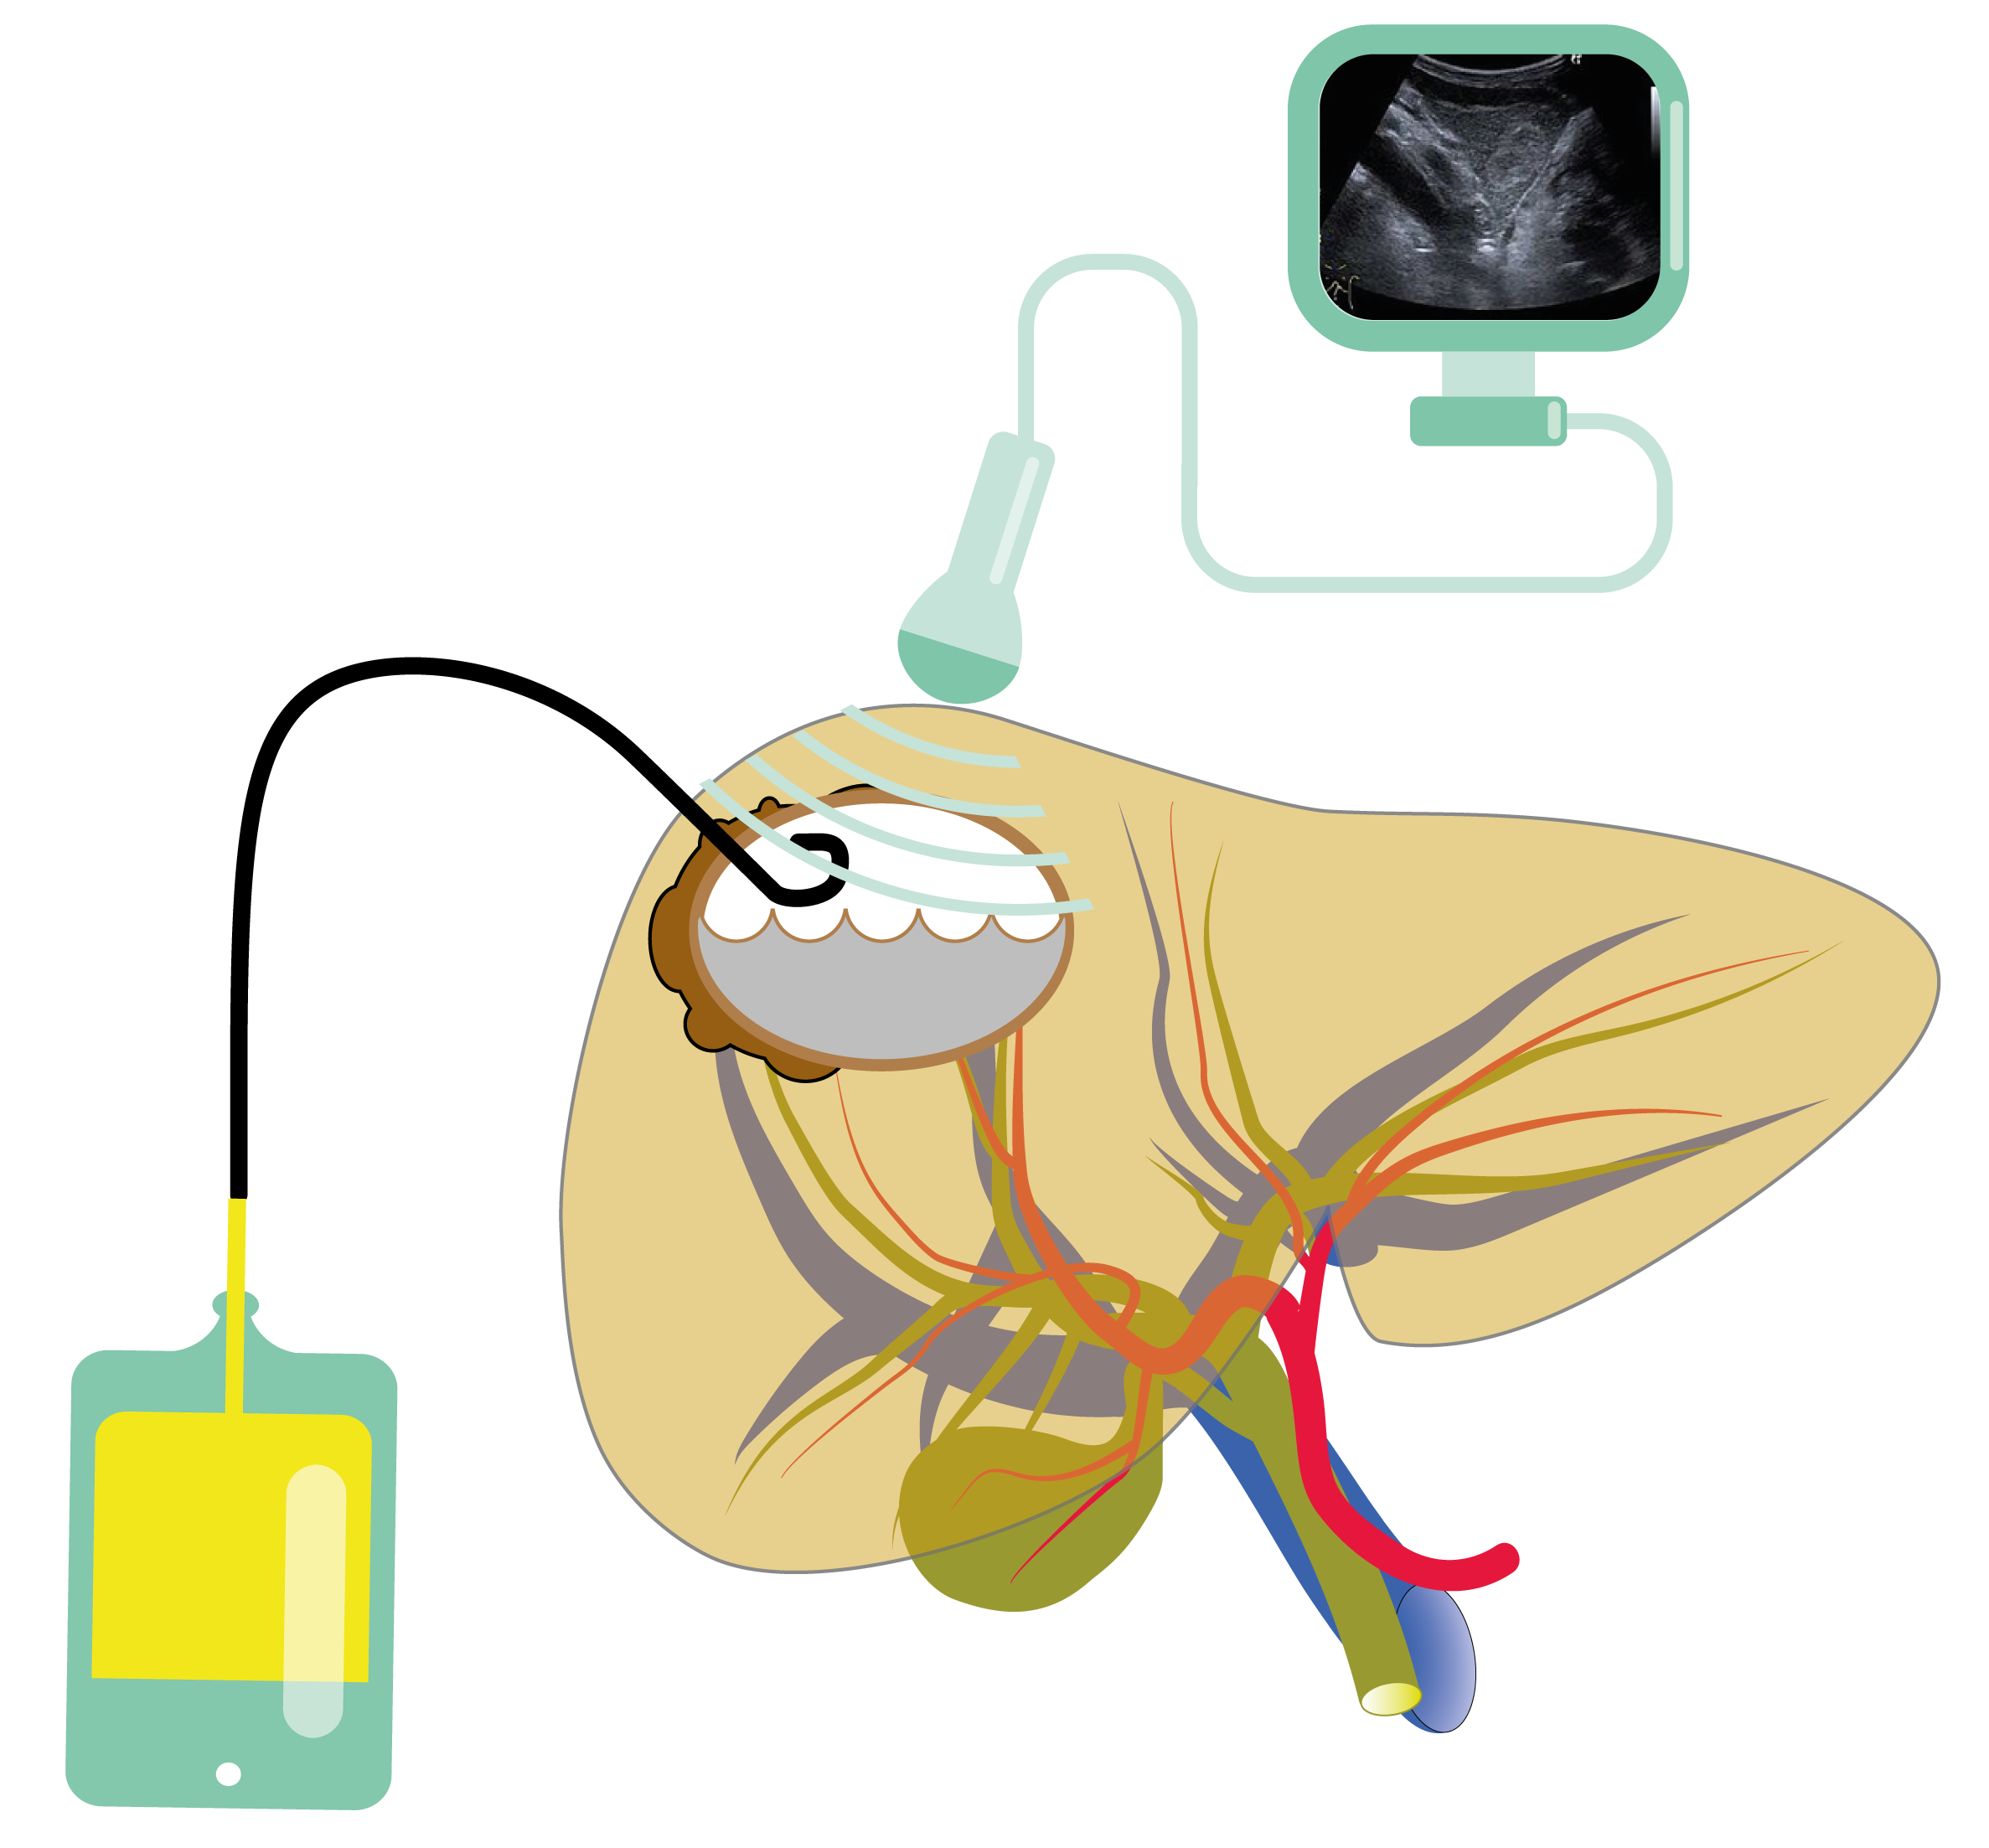
\includegraphics[width=\linewidth]{Figures/US procedures_Drain.png}
            \caption{Дренування абсцесу печінки під контролем ультразвуку}
            \label{fig:goalbladder}
        \end{marginfigure}
        
        
        
        \item біопсія печінки - взяття ділянки тканини печінки або пухлини для подальшого гістологічного дослідження. Використовується для постановки або уточнення діагнозу. Може бути виконана в 2 варіантах - пункційному (під УЗ-контролем) та лапароскопічному (під час діагностичної лапароскопії)
        
        \begin{marginfigure}%
            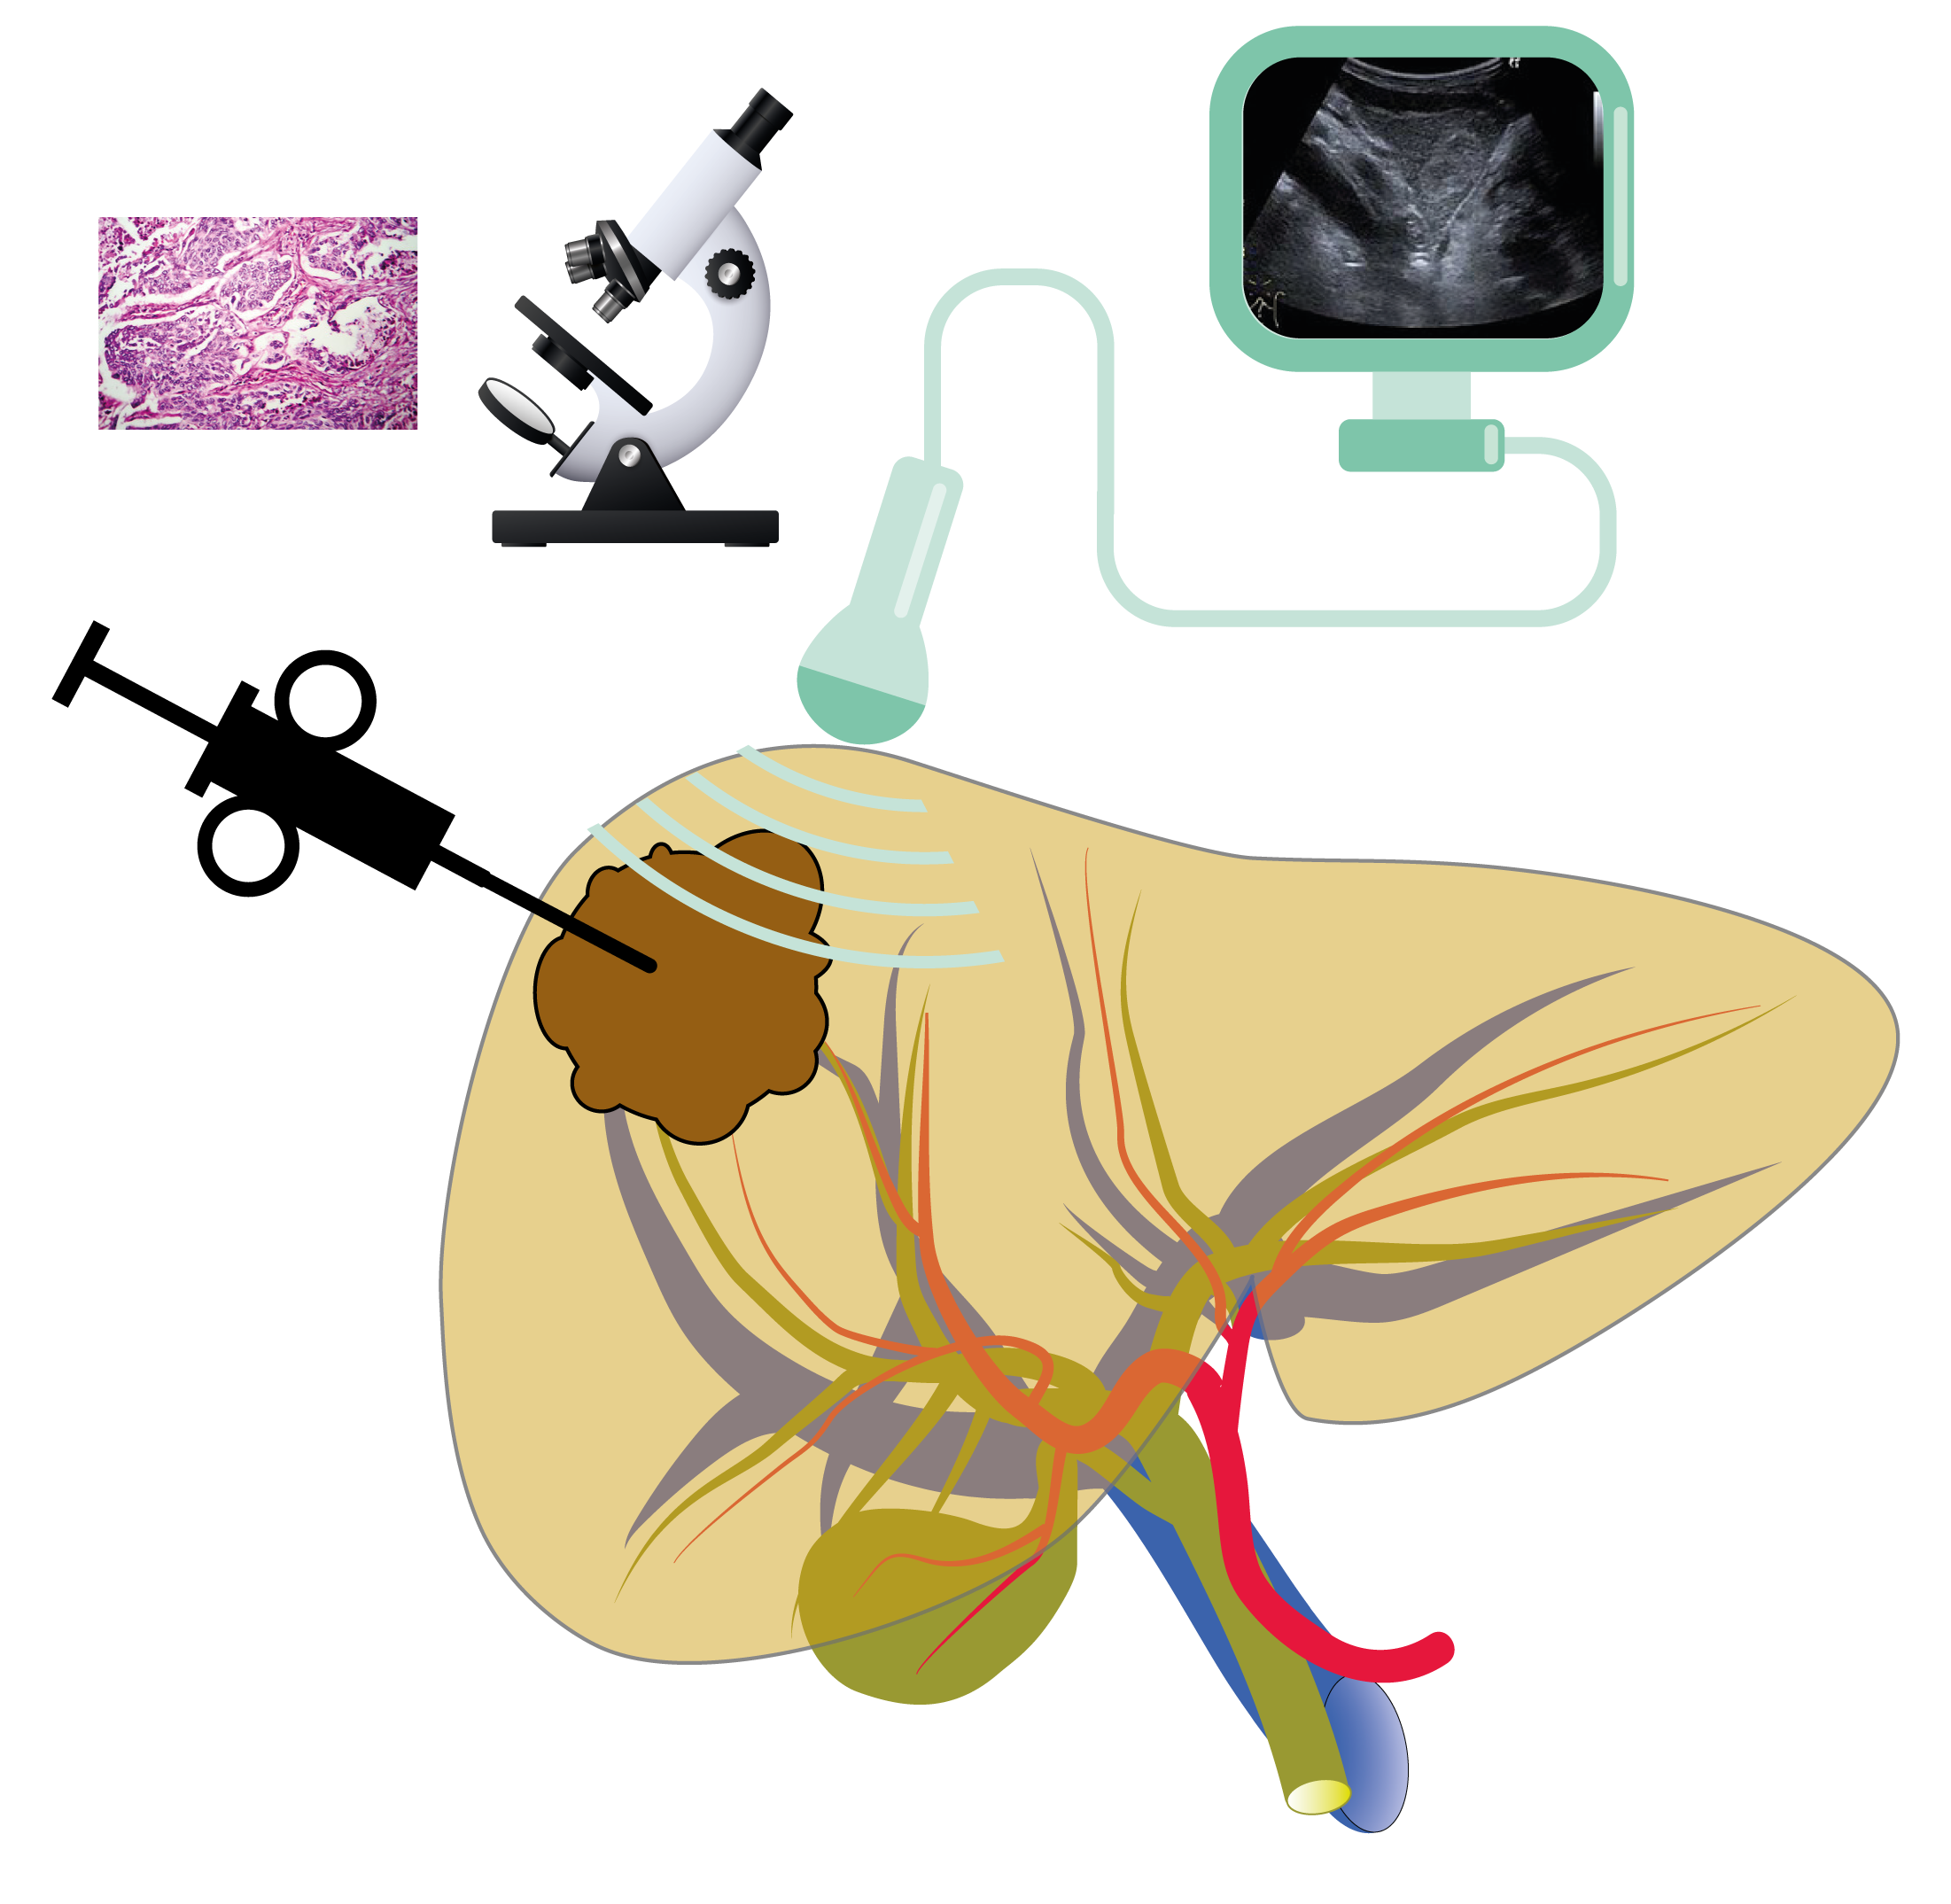
\includegraphics[width=\linewidth]{Figures/US procedures_Biopsy.png}
            \caption{Взяття ділянки пухлини біопсійною голкою під контролем ультразвуку для уточнення діагнозу}
            \label{fig:goalbladder}
        \end{marginfigure}
        
    \end{itemize}
	\item Ендобіліарні, рентгенконтрольовані втручання
	\begin{itemize}
	    \item зовнішнє дренування жовчних шляхів - процедура, під час якої в просвіт жовчного протоку через шкіру встановлюється дренажна трубка по якій далі відходить жовч. Використовується для тимчасової коррекції механічної жовтяниці перед операцією
	    
	    \begin{marginfigure}%
            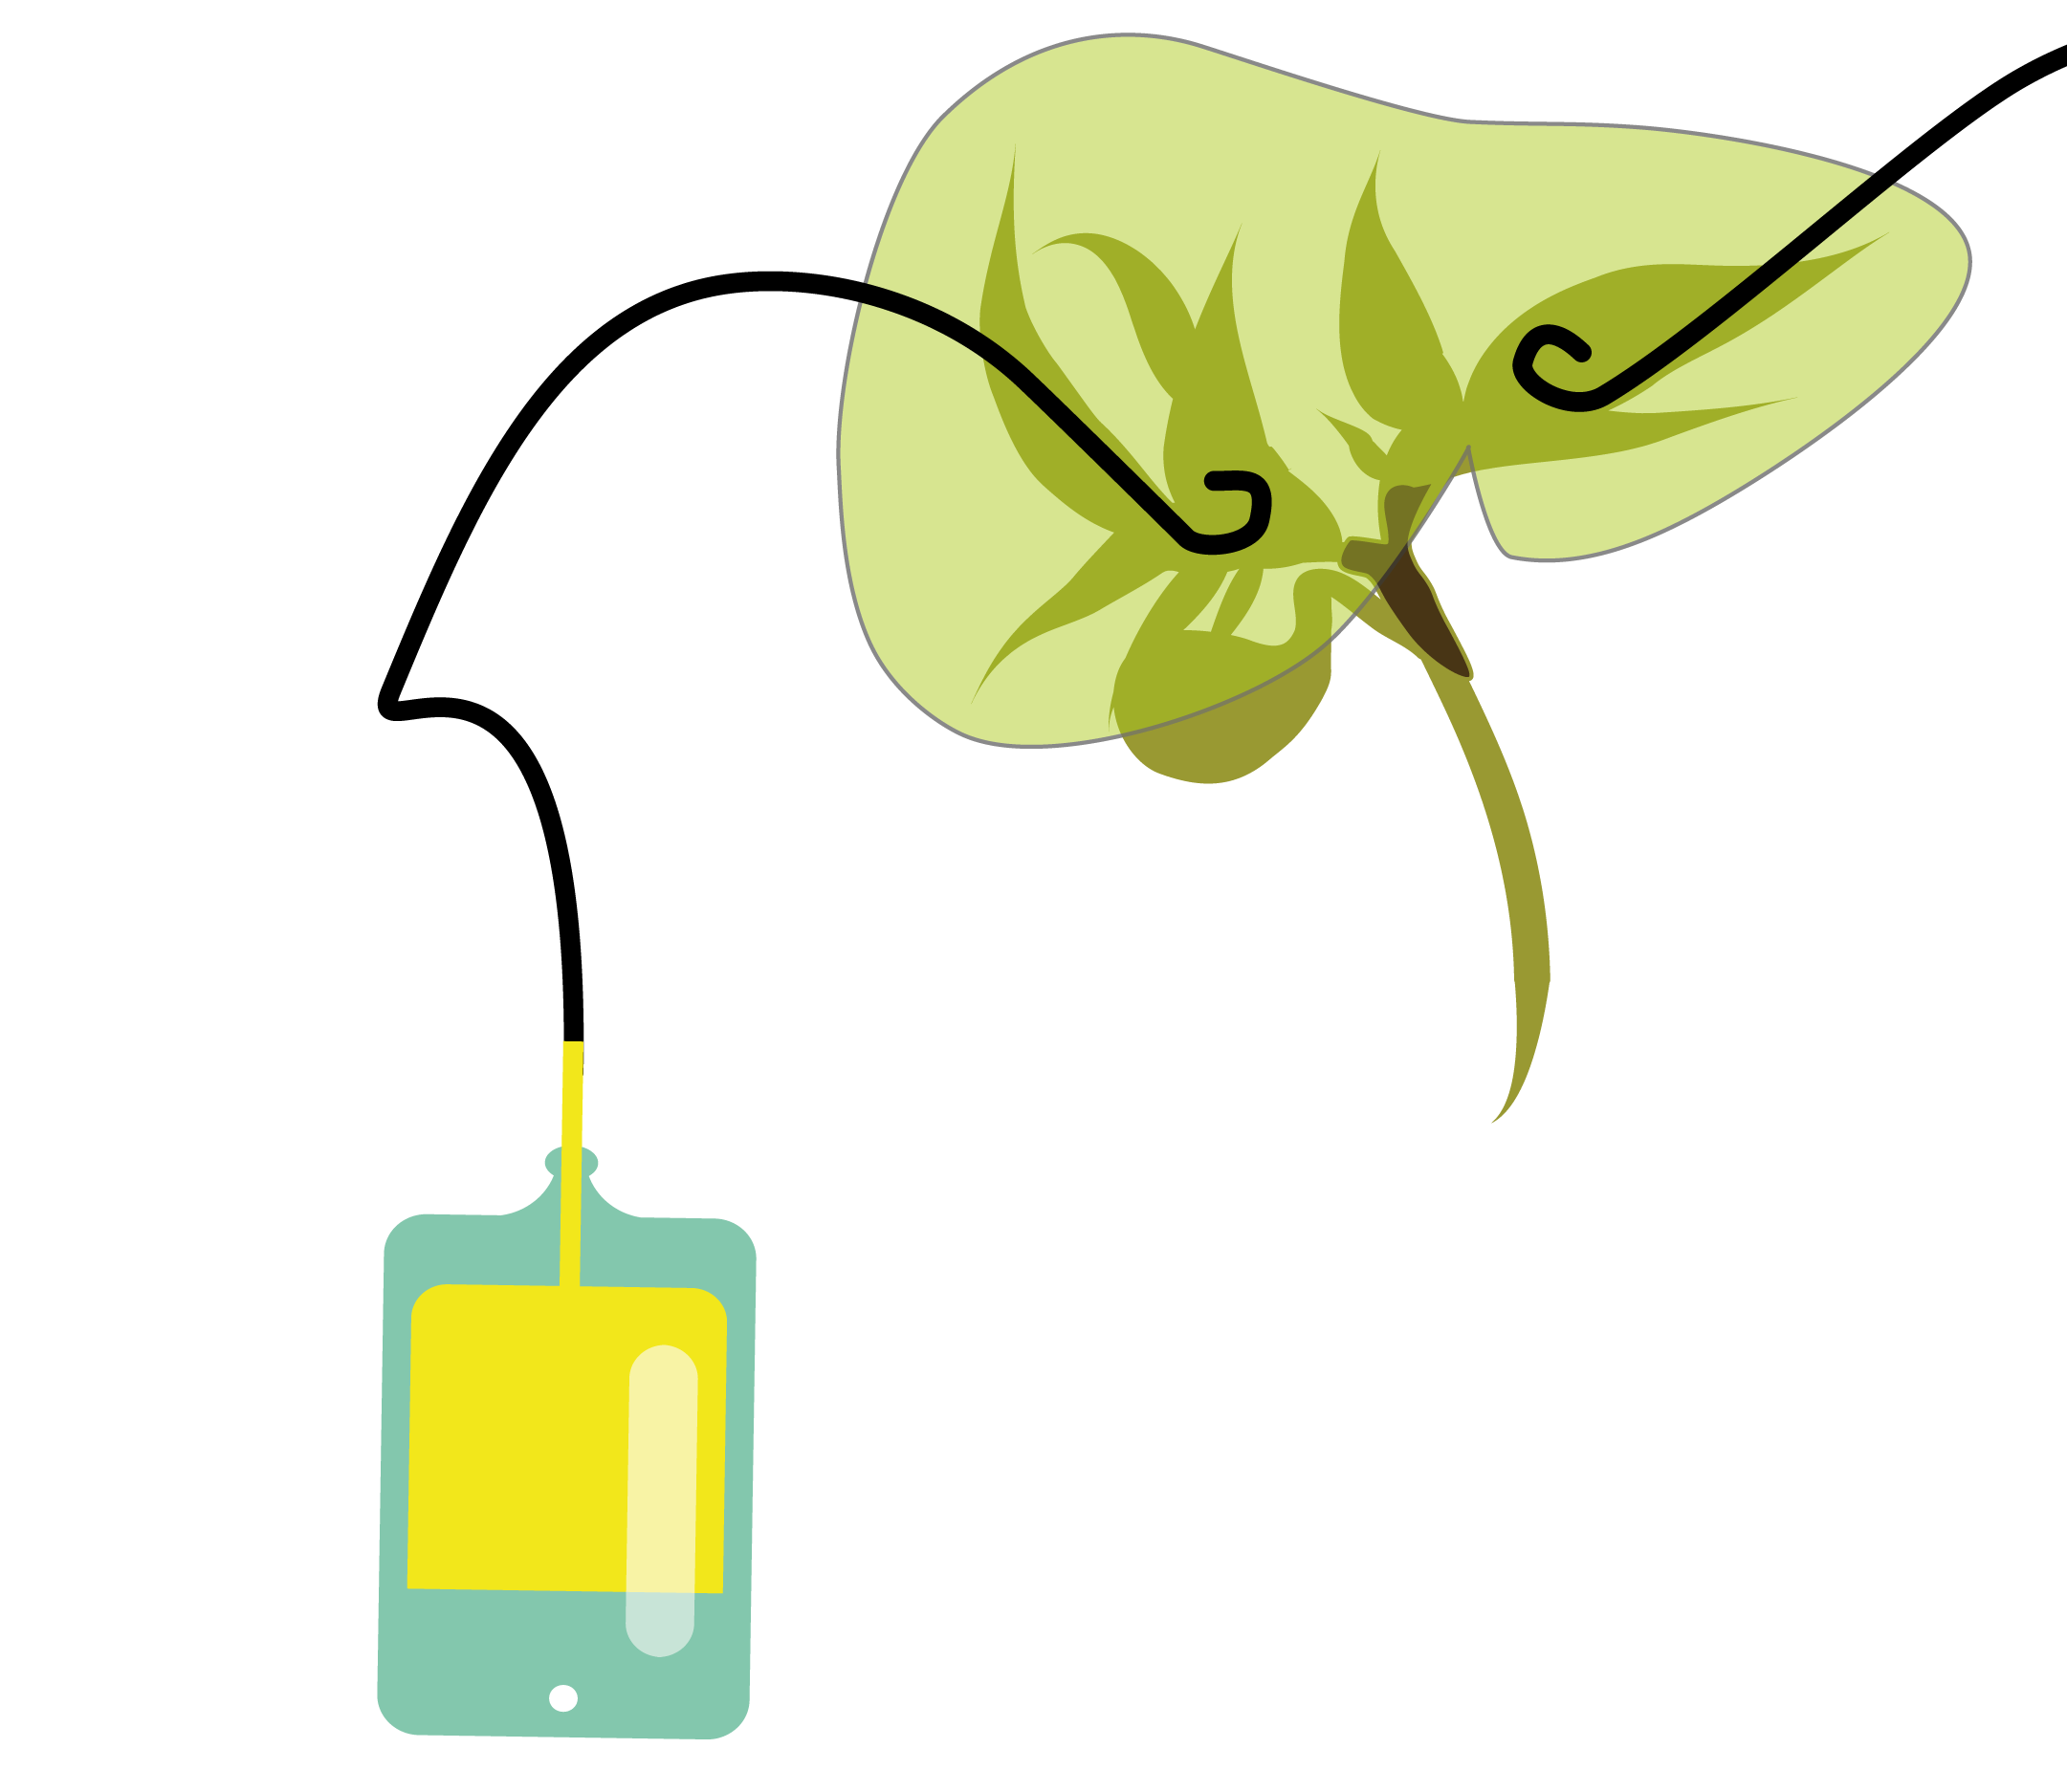
\includegraphics[width=\linewidth]{Figures/PTBD_Liver with drain.png}
            \caption{Встановлення черезшкірних черезпечінкових дренажів жовчних протоків під рентген-контролем для розрішення механічної жовтяниці внаслідок пухлинного процесу}
            \label{fig:goalbladder}
        \end{marginfigure}
	    
	    \item стентування жовчних протоків - процедура, під час якої в просвіт жовчного протоку встановлюється стент - спеціальний постійний розширювач, що дозволяє жовчі проходити повз механічну перепону. Використовується для постійної коррекції механічної жовтяницї
	    
	    \begin{marginfigure}%
            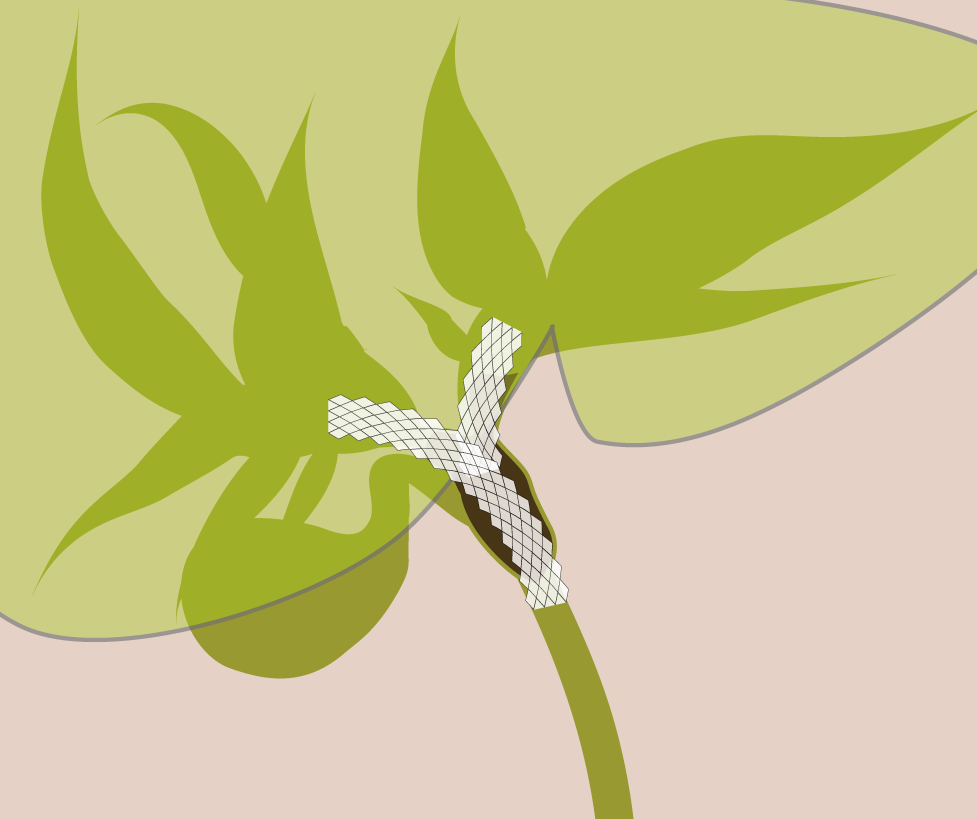
\includegraphics[width=\linewidth]{Figures/Bile duct stent_Stent.png}
            \caption{Встановлення встановлення ендобіліарного стенту для відновлення прохідності жовчних протоків під рентген-контролем}
            \label{fig:goalbladder}
        \end{marginfigure}
	    
	    \item ендоскопічна ретроградна холангіопанкреатографія - методика діагностики та лікування ураженнь жовчних шляхів за допомогою ендоскопа
	\end{itemize}
\end{itemize}